%!TEX root = ../main.tex
\chapter{Introduzione}
\LezioneV{25/02/2021}

Sia $X$ spazio vettoriale normato reale, stiamo chiedendo due cose: combinazioni lineari e la presenza di una norma.

\begin{definition}
    [Norma] Una norma è un operatore $\Vert \cdotp \Vert :X\rightarrow \mathbb{R}$ tale che
    \begin{itemize}
        \item $\Vert x\Vert \geqslant 0,\forall x\in X$ e $\Vert x\Vert =0\Leftrightarrow x=0$
        \item $\Vert \lambda x\Vert =| \lambda | \Vert x\Vert,\forall x\in X,\forall \lambda \in \mathbb{R}$
        \item $\Vert x+y\Vert \leqslant \Vert x\Vert +\Vert y\Vert $
    \end{itemize}
\end{definition}

La norma permette di definire
\begin{itemize}
    \item la distanza $\text{dist}(\x,\y) =\Vert \x-\y\Vert $
    \item le palle aperte $B_{r}(\x) =\{\y\in X:\Vert \x-\y\Vert < r\}$
          \begin{itemize}
              \item di conseguenza la topologia (aperto, chiuso, ...)
          \end{itemize}
\end{itemize}
\begin{nb}
    In $\mathrm{dim}(X) =+\infty $ la nozione di compatto è solo quella definizione
    \begin{equation*}
        \text{chiuso e limitato} \nRightarrow K\ \text{compatto}
    \end{equation*}
\end{nb}
La completezza di uno spazio è importante per costruire successioni approssimanti di una soluzione che \textit{tendano} effettivamente a qualcosa.

Sia $\{x_{n}\}_{n} \subset X$ successione.
\begin{definition}
    Definiamo la convergenza e la continuità
    \begin{enumerate}
        \item $x_{n}\rightarrow \overline{x}$ per $n\rightarrow +\infty $ se $\Vert x_{n} -\overline{x}\Vert \rightarrow 0$
        \item avendo la convergenza, possiamo definire la continuità

              $f:X\rightarrow Y$ è continua se $x_{n}\rightarrow \overline{x} \Rightarrow f(x_{n})\rightarrow f(\overline{x})$
    \end{enumerate}
\end{definition}

\textit{Esercizio.} Dimostrare che la norma $\Vert \cdotp \Vert $ è una funzione continua

Per la disuguaglianza triangolare:
\begin{align*}
    \Vert x\Vert & =\Vert x-x_{0} +x_{0}\Vert                     \\
                 & \leqslant \Vert x-x_{0}\Vert +\Vert x_{0}\Vert
\end{align*}
quindi
\begin{equation*}
    \Big| \Vert x\Vert -\Vert x_{0}\Vert \Big|\leqslant \Vert x-x_{0}\Vert
\end{equation*}
Pertanto se $x\rightarrow x_{0}$ allora $\Vert x\Vert \rightarrow \Vert x_{0}\Vert $.

\begin{definition}
    $\{x_{n}\}_{n\in \mathbb{N}} \subset X$ si dice di Cauchy (o fondamentale) se
    \begin{equation*}
        \Vert x_{n} -x_{m}\Vert \rightarrow 0\ \ \ \ \text{per} \ n,m\rightarrow \infty
    \end{equation*}
\end{definition}
$\{x_{n}\}_{n}$ convergente $\Rightarrow \{x_{n}\}_{n}$ è di Cauchy, infatti
\begin{equation*}
    0\leqslant \Vert x_{n} -x_{m}\Vert =\Vert x_{n} -\overline{x} +\overline{x} -x_{m}\Vert \leqslant \Vert x_{n} -\overline{x}\Vert +\Vert \overline{x} -x_{m}\Vert \rightarrow 0
\end{equation*}
questa è la parte inutile, è più utile il contrario, vedere il comportamento delle approssimazioni e dedurre se c'è convergenza a qualcosa! In generale non è vero che una successione di Cauchy è convergente, per questo motivo lavoriamo in Spazi di Banach.
\begin{definition}
    Se ``di Cauchy'' implica convergente, allora $X$ è completo.
\end{definition}
\begin{definition}
    $X$ si dice Spazio di Banach se è uno spazio vettoriale normato e completo rispetto a quella norma.
\end{definition}
Esempi di spazi di Banach.
\begin{itemize}
    \item $\mathbb{R}^{n}$ con la norma euclidea è completo
    \item $L^{p}(\Omega),\Omega \subset \mathbb{R}^{n}$ dominio\footnote{cioè aperto e connesso.} con la norma
          \begin{equation*}
              \Vert u\Vert _{L^{p}(\Omega)} =\left(\int _{\Omega }| u| ^{p} \dx\right)^{1/p} \ \ 1\leqslant p< \infty
          \end{equation*}
    \item $C(\overline{\Omega })$, con $\Omega $ limitato con la norma
          \begin{equation*}
              \Vert u\Vert _{C(\overline{\Omega })} =\max_{\overline{\Omega }}| u|
          \end{equation*}
\end{itemize}
\begin{definition}
    Supponiamo di avere due norme $\Vert \cdotp \Vert _{1} :X\rightarrow \mathbb{R}$, $\Vert \cdotp \Vert _{2} :X\rightarrow \mathbb{R}$. Si dicono \textbf{equivalenti} se inducono la stessa convergenza, cioè se $\exists 0< c_{1} \leqslant c_{2}$, non dipendenti da $x$, tali che
    \begin{equation*}
        c_{1}\Vert x\Vert _{1} \leqslant \Vert x\Vert _{2} \leqslant c_{2}\Vert x\Vert _{1} \ \ \forall x\in X
    \end{equation*}
\end{definition}
\begin{nb}
    In $\mathbb{R}^{n}$ non abbiamo insistito su questa cosa perché tutte le norme sono equivalenti, gli spazi sono tutti isomorfi.
\end{nb}
\textit{Esempio.}

Consideriamo lo spazio delle funzioni continue in $\displaystyle [ -1,1]$
\begin{equation*}
    X=C([ -1,1])
\end{equation*}
e vediamolo come sottospazio di $\displaystyle L^{2}$
\begin{equation*}
    X\subset L^{2}([ -1,1])
\end{equation*}
Possiamo scegliere due diverse norme, la norma delle funzioni continue, ovvero il massimo, oppure la norma di $\displaystyle L^{2}$.
\begin{equation*}
    \Vert \cdotp \Vert _{C([ -1,1])} \ \ \ \ \Vert \cdotp \Vert _{L^{2}([ -1,1])}
\end{equation*}
\begin{itemize}
    \item Con la norma $\displaystyle \Vert \cdotp \Vert _{C([ -1,1])}$

          $X$ è uno spazio \textbf{completo}, per dirlo ci serve far vedere che tutte le successioni di Cauchy sono convergenti. In particolare, per ogni $x$ fissato si hanno delle successioni di numeri in $\displaystyle \mathbb{R}$, che è completo, quindi il candidato limite della successione di Cauchy è il limite puntuale $\displaystyle f(x)$
          \begin{gather*}
              \underbrace{\forall \varepsilon  >0,\exists M >0:\Vert f_{n} -f_{m}\Vert _{C([ -1,1])} < \varepsilon \ \text{per} \ n,m\geqslant M}_{\text{Cauchy}}\\
              \text{allora}\\
              \begin{aligned}
                  \forall m >M,\forall x\in [ -1,1],\quad |f(x) -f_{m}(x) | & =\lim _{n\rightarrow \infty } |f_{n}(x) -f_{m}(x) |                        \\
                                                                            & \leqslant \lim _{n\rightarrow \infty }\max_{[ -1,1]} |f_{n}(x) -f_{m}(x) | \\
                                                                            & =\lim _{n\rightarrow \infty }\Vert f_{n} -f_{m}\Vert _{C([ -1,1])}         \\
                                                                            & \leqslant \lim _{n\rightarrow \infty } \varepsilon =\varepsilon
              \end{aligned}
          \end{gather*}
    \item Con la norma $\displaystyle \Vert \cdotp \Vert _{L^{2}([ -1,1])}$

          $X$ \textbf{non è completo}, perché possiamo trovare una successione di Cauchy che non converge (o meglio, che converge a qualcosa che non appartiene allo spazio).

          Consideriamo la seguente successione
          \begin{equation*}
              v_{n}(x) =
              \begin{cases}
                  0,  & -1\leqslant x\leqslant 0           \\
                  nx, & 0\leqslant x\leqslant \frac{1}{n}  \\
                  1,  & \frac{1}{n} \leqslant x\leqslant 1
              \end{cases}
          \end{equation*}

          \begin{figure}[htpb]
              \centering

              \tikzset{every picture/.style={line width=0.75pt}} %set default line width to 0.75pt        

              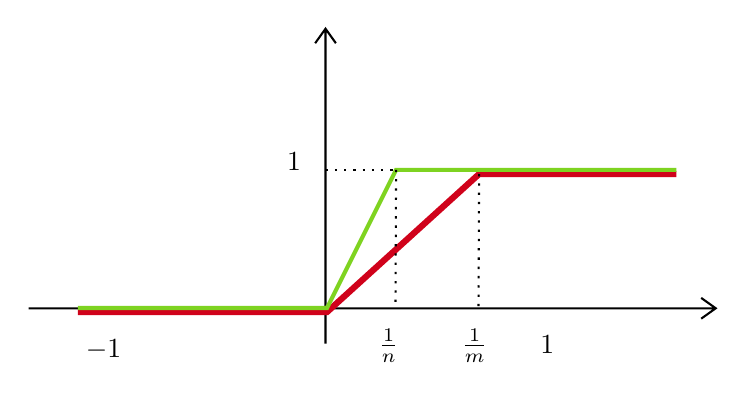
\begin{tikzpicture}[x=0.75pt,y=0.75pt,yscale=-1,xscale=1]
                  %uncomment if require: \path (0,197); %set diagram left start at 0, and has height of 197

                  %Shape: Axis 2D [id:dp7510112278083159] 
                  \draw  (141,140.7) -- (472,140.7)(284,6) -- (284,157.7) (465,135.7) -- (472,140.7) -- (465,145.7) (279,13) -- (284,6) -- (289,13)  ;
                  %Straight Lines [id:da35643943970375824] 
                  \draw [color={rgb, 255:red, 208; green, 2; blue, 27 } ,draw opacity=1 ][line width=2.25]    (453,76) -- (358,76) -- (284.7,142.53) -- (164.7,142.53) ;
                  %Straight Lines [id:da14888962981095388] 
                  \draw  [dash pattern={on 0.84pt off 2.51pt}]  (358,76) -- (357.7,142.53) ;
                  %Straight Lines [id:da7820546278212102] 
                  \draw [color={rgb, 255:red, 126; green, 211; blue, 33 } ,draw opacity=1 ][line width=1.5]    (453,74) -- (318,74) -- (284.7,140.53) -- (164.7,140.53) ;
                  %Straight Lines [id:da933791757163982] 
                  \draw  [dash pattern={on 0.84pt off 2.51pt}]  (318,74) -- (317.7,140.53) ;
                  %Straight Lines [id:da44978431803839936] 
                  \draw  [dash pattern={on 0.84pt off 2.51pt}]  (284,74) -- (318,74) ;

                  % Text Node
                  \draw (167,154.4) node [anchor=north west][inner sep=0.75pt]    {$-1$};
                  % Text Node
                  \draw (386,152.4) node [anchor=north west][inner sep=0.75pt]    {$1$};
                  % Text Node
                  \draw (348,149.4) node [anchor=north west][inner sep=0.75pt]    {$\frac{1}{m}$};
                  % Text Node
                  \draw (308,149.4) node [anchor=north west][inner sep=0.75pt]    {$\frac{1}{n}$};
                  % Text Node
                  \draw (264,64.4) node [anchor=north west][inner sep=0.75pt]    {$1$};


              \end{tikzpicture}

          \end{figure}
          \FloatBarrier

          Verifichiamo che è di Cauchy, supponiamo $\displaystyle m\leqslant n$
          \begin{align*}
              \Vert v_{n} -v_{m}\Vert _{2}^{2} & =\int _{-1}^{1}(v_{n}(x) -v_{m}(x))^{2} \dx                                            \\
                                               & =\cancel{\int _{-1}^{0}} +\int _{0}^{1/n} +\int _{1/n}^{1/m} +\cancel{\int _{1/m}^{1}} \\
                                               & =\int _{0}^{1/n}(n-m)^{2} x^{2} \dx+\int _{1/n}^{1/m}(1-mx)^{2} \dx\rightarrow 0
          \end{align*}Tuttavia è convergente a Heaviside, che non è continua.

          Se inoltre consideriamo la norma solita delle funzioni continue notiamo che non è nemmeno di Cauchy
          \begin{equation*}
              \Vert v_{n} -v_{m}\Vert _{C([ -1,1])} =\max_{x\in [ -1,1]}(v_{n}(x) -v_{m}(x)) =1-\frac{m}{n} \nrightarrow 0
          \end{equation*}per $n,m\rightarrow \infty $, infatti se scegliamo $n=2m$ il limite tenderebbe a $1/2$.
\end{itemize}

In questo esempio:
\begin{itemize}
    \item Con $\displaystyle \Vert \cdotp \Vert _{L^{2}}$
          \begin{itemize}
              \item La successione è di Cauchy ma non converge, quindi non è completo.
          \end{itemize}
    \item Con $\Vert \cdotp \Vert _{C}$
          \begin{itemize}
              \item La successione non è di Cauchy.
              \item In generale lo spazio è completo.
          \end{itemize}
    \item Deduciamo anche che le due norme non sono equivalenti, dato che inducono convergenze diverse sulla stessa successione.
\end{itemize}

\begin{definition}
    [Prodotto scalare] $(\cdotp,\cdotp) :X\times X\rightarrow \mathbb{R}$ tale che
    \begin{itemize}
        \item $(v,v) \geqslant 0$ e $(v,v) =0\Leftrightarrow v=0$
        \item $(u,v) =(v,u),\forall u,v\in X$
        \item $(\lambda _{1} u_{1} +\lambda _{2} u_{2},v) =\lambda _{1}(u_{1},v) +\lambda _{2}(u_{2},v),\forall \lambda _{1},\lambda _{2} \in \mathbb{R},\forall u_{1},u_{2},v\in X$
    \end{itemize}
\end{definition}
\begin{definition}
    Norma indotta dal prodotto scalare
    \begin{equation*}
        \Vert v\Vert =\sqrt{(v,v)}
    \end{equation*}
\end{definition}
Esercizio. Verificare che il prodotto scalare è continuo rispetto alla norma indotta e che $\Vert \cdotp \Vert $ è una norma.
\begin{theorem}
    Alcune proposizioni
    \begin{enumerate}
        \item Cauchy-Schwarz $| (u,v)| \leqslant \Vert u\Vert \cdotp \Vert v\Vert $
        \item Identità del parallelogramma\footnote{la somma dei quadrati sulle diagonali è uguale alla somma dei quadrati su tutti i lati.} $\Vert u+v\Vert ^{2} +\Vert u-v\Vert ^{2} =2\Vert u\Vert ^{2} +2\Vert v\Vert ^{2}$, vale solo se la norma è indotta da un prodotto scalare
    \end{enumerate}
\end{theorem}
\begin{definition}
    Uno spazio vettoriale $X$, con prodotto scalare, che sia completo rispetto alla norma indotta dal prodotto scalare si dice \textbf{Spazio di Hilbert}.
\end{definition}
\textit{Esempi.}

$\mathbb{R}^{n},L^{2}(\Omega)$ con la norma indotta dal prodotto scalare $(u,v)_{L^{2}(\Omega)} =\int _{\Omega } uv\dx$

In uno spazio con prodotto scalare possiamo definire l'\textbf{ortogonalità}
\begin{equation*}
    u\perp v\Leftrightarrow (u,v) =0
\end{equation*}
\section{Approssimazione di vettori (Teorema delle Proiezioni)}

Chiameremo $H$ un generico spazio di Hilbert. Considerando $H$ e $V\subset H$ sottospazio\footnote{$u,v\in V\Rightarrow \lambda u+\mu v\in V$.}, $x\in H$, vogliamo trovare il vettore di $V$ che meglio approssima $x$. Stiamo cercando $\overline{v} \in V$ tale che
\begin{equation*}
    \Vert x-\overline{v}\Vert =\inf_{v\in V}\Vert x-v\Vert
\end{equation*}

\begin{figure}[htpb]
    \centering

    \tikzset{every picture/.style={line width=0.75pt}} %set default line width to 0.75pt        

    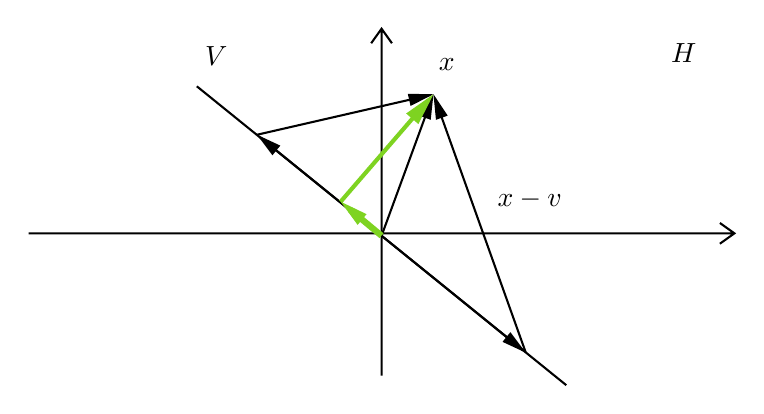
\begin{tikzpicture}[x=0.75pt,y=0.75pt,yscale=-1,xscale=1]
        %uncomment if require: \path (0,198); %set diagram left start at 0, and has height of 198

        %Straight Lines [id:da9073640143708681] 
        \draw    (301,113.41) -- (242.55,66.01) ;
        \draw [shift={(241,64.75)}, rotate = 399.03999999999996] [fill={rgb, 255:red, 0; green, 0; blue, 0 }  ][line width=0.08]  [draw opacity=0] (12,-3) -- (0,0) -- (12,3) -- cycle    ;
        %Shape: Axis 2D [id:dp9737576348755399] 
        \draw  (131,112.25) -- (471,112.25)(301,13.66) -- (301,180.75) (464,107.25) -- (471,112.25) -- (464,117.25) (296,20.66) -- (301,13.66) -- (306,20.66)  ;
        %Straight Lines [id:da5543961945984461] 
        \draw    (212,41.41) -- (390,185.41) ;
        %Straight Lines [id:da7822239085129437] 
        \draw    (301,113.41) -- (325.31,47.13) ;
        \draw [shift={(326,45.25)}, rotate = 470.14] [fill={rgb, 255:red, 0; green, 0; blue, 0 }  ][line width=0.08]  [draw opacity=0] (12,-3) -- (0,0) -- (12,3) -- cycle    ;
        %Straight Lines [id:da5022645915295285] 
        \draw    (370.5,169.75) -- (326.67,47.13) ;
        \draw [shift={(326,45.25)}, rotate = 430.33000000000004] [fill={rgb, 255:red, 0; green, 0; blue, 0 }  ][line width=0.08]  [draw opacity=0] (12,-3) -- (0,0) -- (12,3) -- cycle    ;
        %Straight Lines [id:da8728054276938597] 
        \draw    (241,64.75) -- (324.05,45.7) ;
        \draw [shift={(326,45.25)}, rotate = 527.0799999999999] [fill={rgb, 255:red, 0; green, 0; blue, 0 }  ][line width=0.08]  [draw opacity=0] (12,-3) -- (0,0) -- (12,3) -- cycle    ;
        %Straight Lines [id:da7420419315205793] 
        \draw [color={rgb, 255:red, 126; green, 211; blue, 33 } ,draw opacity=1 ][line width=1.5]    (281.29,97) -- (323.38,48.28) ;
        \draw [shift={(326,45.25)}, rotate = 490.83] [fill={rgb, 255:red, 126; green, 211; blue, 33 } ,fill opacity=1 ][line width=0.08]  [draw opacity=0] (15.6,-3.9) -- (0,0) -- (15.6,3.9) -- cycle    ;
        %Straight Lines [id:da5034396510582315] 
        \draw [color={rgb, 255:red, 126; green, 211; blue, 33 } ,draw opacity=1 ][line width=2.25]    (301,113.41) -- (285.9,100.84) ;
        \draw [shift={(281.29,97)}, rotate = 399.77] [fill={rgb, 255:red, 126; green, 211; blue, 33 } ,fill opacity=1 ][line width=0.08]  [draw opacity=0] (13.44,-3.36) -- (0,0) -- (13.44,3.36) -- cycle    ;
        %Straight Lines [id:da8018205092868931] 
        \draw    (301,113.41) -- (368.95,168.49) ;
        \draw [shift={(370.5,169.75)}, rotate = 219.03] [fill={rgb, 255:red, 0; green, 0; blue, 0 }  ][line width=0.08]  [draw opacity=0] (12,-3) -- (0,0) -- (12,3) -- cycle    ;

        % Text Node
        \draw (439,19.4) node [anchor=north west][inner sep=0.75pt]    {$H$};
        % Text Node
        \draw (214.5,20.9) node [anchor=north west][inner sep=0.75pt]    {$V$};
        % Text Node
        \draw (327.14,26.61) node [anchor=north west][inner sep=0.75pt]    {$x$};
        % Text Node
        \draw (355.43,90.04) node [anchor=north west][inner sep=0.75pt]    {$x-v$};


    \end{tikzpicture}

\end{figure}
\FloatBarrier

$\displaystyle \overline{v}$ è la proiezione su $V$ di $x$, che indicheremo come $P_{V} x$, è l'elemento di minima distanza (\textit{se esiste}).
\begin{itemize}
    \item in $\mathrm{dim} < +\infty $ esiste sempre (Gram-Schmidt).
    \item in $\mathrm{dim} =\infty $ non è detto, servono ipotesi in più, che sia \textbf{chiuso}.
\end{itemize}

Nel caso di prima possiamo approssimare Heaviside con le approssimanti introdotte, ma non c'è \textit{la migliore}, questo ci dice che le funzioni continue non sono un sottospazio \textit{chiuso}.

\LezioneV{04/03/2021}
\begin{theorem}
    [delle Proiezioni] Sia $H$ di Hilbert, $V$ sottospazio vettoriale di $H$ \textbf{chiuso}\footnote{in senso topologico, deve contenere tutti i suoi punti di frontiera.}, $x\in H$. Allora $\exists !P_{V} x\in V$ tale che
    \begin{equation*}
        \Vert P_{V} x-x\Vert =\inf_{v\in V}\Vert v-x\Vert
    \end{equation*}

    \textbf{Inoltre:}
    \begin{enumerate}
        \item $\displaystyle x\in V\ \Leftrightarrow \ x=P_{V} x$
        \item Definendo $\displaystyle Q_{V} x=x-P_{V} x$ si ha $(Q_{V} x,v) =0\ \forall v\in V$, cioè $\displaystyle Q_{V} x\in V^{\bot }$

              Inoltre vale un teorema di Pitagora generalizzato: $\Vert x\Vert ^{2} =\Vert P_{V} x\Vert ^{2} +\Vert Q_{V} x\Vert ^{2}$.
    \end{enumerate}
\end{theorem}
\begin{nb}
    Se $\displaystyle \mathrm{dim} H\mathrm{=+\infty }$ non è detto che i sottospazi siano chiusi, a differenza di spazi a dimensione finita, però se
    \begin{equation*}
        \mathrm{dim} V< +\infty,\ V\subset H\ \ \Rightarrow \ V\ \text{chiuso}
    \end{equation*}
    e in ogni caso $\displaystyle V^{\bot }$è chiuso, infatti:
    \begin{equation*}
        \text{se} \ y_{n}\rightarrow y,\ \{y_{n}\} \subset V^{\bot } \ \ \Rightarrow \ \ \forall x\in V,(y,x) =\lim _{n\rightarrow \infty }(y_{n} ,x) =0\ \ \Rightarrow \ \ y\in V^{\bot }
    \end{equation*}
\end{nb}

\begin{dimostrazione}
    Dimostriamo per passi, prima l'esistenza, poi l'unicità e infine i vari punti aggiuntivi.
    \begin{itemize}
        \item Esistenza
              \begin{equation*}
                  d=\inf_{v\in V}\Vert v-x\Vert,\ d\geqslant 0
              \end{equation*}

              ovvero, per definizione di $\inf$
              \begin{enumerate}
                  \item $\displaystyle \Vert v-x\Vert \geqslant d,\ \forall v\in V$
                  \item $\displaystyle \forall \varepsilon \ \exists v_{\varepsilon } \in V$ tale che $\displaystyle \Vert v_{\varepsilon } -x\Vert \leqslant d+\varepsilon $ \ $ $
              \end{enumerate}

              uso la definizione per costruire una ``successione minimizzante''
              \begin{equation}
                  (v_{n})_{n\in \mathbb{N}} \subset V:\ d\leqslant \Vert x-v_{n}\Vert \leqslant d+\frac{1}{n} \ \ \left(\varepsilon =\frac{1}{n},\ n\in \mathbb{N}\right)
                  \label{eq:teo-proiez-suc-min}
              \end{equation}

              voglio dimostrare che la successione converge. Per farlo devo prima dimostrare che è una successione di Cauchy. Uso l'identità del parallelogramma riscritta nel seguente modo
              \begin{equation*}
                  \Vert a-b\Vert ^{2} =2\Vert a\Vert ^{2} +2\Vert b\Vert ^{2} -\Vert a+b\Vert ^{2}
              \end{equation*}

              con $\displaystyle a=v_{n} -x$, $\displaystyle b=v_{m} -x$, i termini dell'identità diventano:
              \begin{equation*}
                  \begin{array}{ l }
                      \Vert a-b\Vert ^{2} =\Vert v_{n} -v_{m}\Vert ^{2} \\
                      \Vert a+b\Vert ^{2} =\Vert v_{n} +v_{m} -2x\Vert ^{2} =4\bigg\Vert \underbrace{\frac{v_{n} +v_{m}}{2}}_{\in V} -x\bigg\Vert ^{2} \geqslant 4d^{2}
                  \end{array}
              \end{equation*}

              dove l'ultima disuguaglianza vale perché $\Vert v-x\Vert \geqslant d,\ \forall v\in V$ (definizione di $\inf$) e $\displaystyle \frac{v_{n} +v_{m}}{2} \in V$, essendo $V$ un sottospazio.

              La norma di $a$ e di $b$ tenderà a $d$ per il teorema dei carabinieri e per \eqref{eq:teo-proiez-suc-min}. Sostituendo nell'identità
              \begin{align*}
                  0 & \leqslant \Vert v_{n} -v_{m}\Vert ^{2}                                                                       \\
                    & =2\Vert v_{n} -x\Vert ^{2} +2\Vert v_{m} -x\Vert ^{2} -4\left\Vert \frac{v_{n} +v_{m}}{2} -x\right\Vert ^{2} \\
                    & \leqslant 2\Vert v_{n} -x\Vert ^{2} +2\Vert v_{m} -x\Vert ^{2} -4d^{2}                                       \\
                    & \xrightarrow[n,m\rightarrow \infty ]{} 2d^{2} +2d^{2} -4d^{2} =0
              \end{align*}

              Quindi la mia successione minimizzante è di Cauchy. Ma poiché $H$ è di Hilbert, ogni successione di Cauchy è convergente
              \begin{equation*}
                  v_{n}\xrightarrow{n\rightarrow \infty }\overline{v} \in H
              \end{equation*}

              \textbf{e poiché $V$ è chiuso,} $\overline{v} \in V$. Allora prendendo la definizione della mia successione \begin{equation*}
                  d\leqslant \Vert x-v_{n}\Vert \leqslant d+\frac{1}{n}
              \end{equation*}

              e facendone il limite per $n\rightarrow \infty $ ottengo, per continuità della norma
              \begin{equation*}
                  d\leqslant \Vert x-\overline{v}\Vert \leqslant d
              \end{equation*}

              Definisco la proiezione di $x$ su $V$: $\boxed{P_{V} x=\overline{v}}$
        \item Unicità

              Per assurdo
              \begin{equation*}
                  \overline{v},\overline{w} \in V,\ \ \Vert \overline{v} -x\Vert =\Vert \overline{w} -x\Vert =d
              \end{equation*}

              Usando l'identità del parallelogramma con $a=\overline{v} -x$, $b=\overline{w} -x$:
              \begin{equation*}
                  \Vert \overline{v} -\overline{w}\Vert ^{2} +\Vert \overline{v} +\overline{w} -2x\Vert ^{2} =4d^{2}
              \end{equation*}

              Sfruttando gli stessi passaggi dell'esistenza osservo che $\Vert \overline{v} +\overline{w} -2x\Vert ^{2} \geqslant 4d^{2}$. Allora perchè l'identità sia soddisfatta deve essere $\Vert \overline{v} -\overline{w}\Vert ^{2} \leqslant 0$, ma quindi $\Vert \overline{v} -\overline{w}\Vert ^{2} =0$, infine per proprietà della norma:
              \begin{equation*}
                  \overline{v} =\overline{w}
              \end{equation*}
        \item Inoltre (punto 1)\\
              Conseguenza banale, se $x\in V$
              \begin{equation*}
                  d=\inf_{v\in V}\Vert v-x\Vert =0
              \end{equation*}
              quindi come prima $\Vert x-P_{V} x\Vert =0\ \Rightarrow \ x=P_{V} x$
        \item Inoltre (punto 2)\\
              Definendo $Q_{V} x=x-P_{V} x$, osserviamo che $\forall v\in V,\ t\in \mathbb{R} \Longrightarrow (P_{V} x-tv) \in V$




              \begin{figure}[H]
                  \centering

                  \tikzset{every picture/.style={line width=0.75pt}} %set default line width to 0.75pt        

                  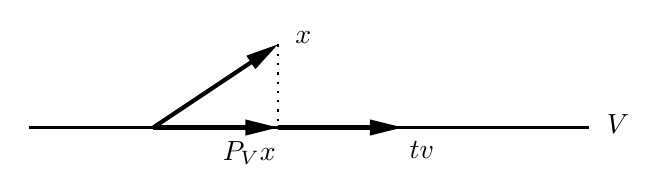
\begin{tikzpicture}[x=0.75pt,y=0.75pt,yscale=-1,xscale=1]
                      %uncomment if require: \path (0,98); %set diagram left start at 0, and has height of 98

                      %Straight Lines [id:da1966060419350555] 
                      \draw [color={rgb, 255:red, 0; green, 0; blue, 0 } ,draw opacity=1 ]   (90,60) -- (360,60) ;
                      %Straight Lines [id:da864357839898725] 
                      \draw [line width=1.5]    (150,60) -- (206,60) ;
                      \draw [shift={(210,60)}, rotate = 180] [fill={rgb, 255:red, 0; green, 0; blue, 0 }  ][line width=0.08]  [draw opacity=0] (15.6,-3.9) -- (0,0) -- (15.6,3.9) -- cycle    ;
                      %Straight Lines [id:da07495012975809501] 
                      \draw [line width=1.5]    (210,60) -- (266,60) ;
                      \draw [shift={(270,60)}, rotate = 180] [fill={rgb, 255:red, 0; green, 0; blue, 0 }  ][line width=0.08]  [draw opacity=0] (15.6,-3.9) -- (0,0) -- (15.6,3.9) -- cycle    ;
                      %Straight Lines [id:da21049925432833838] 
                      \draw [line width=1.5]    (150,60) -- (206.67,22.22) ;
                      \draw [shift={(210,20)}, rotate = 506.31] [fill={rgb, 255:red, 0; green, 0; blue, 0 }  ][line width=0.08]  [draw opacity=0] (15.6,-3.9) -- (0,0) -- (15.6,3.9) -- cycle    ;
                      %Straight Lines [id:da673978991154291] 
                      \draw  [dash pattern={on 0.84pt off 2.51pt}]  (210,20) -- (210,60) ;

                      % Text Node
                      \draw (182,65.4) node [anchor=north west][inner sep=0.75pt]    {$P_{V} x$};
                      % Text Node
                      \draw (272,65.4) node [anchor=north west][inner sep=0.75pt]    {$tv$};
                      % Text Node
                      \draw (217,12.4) node [anchor=north west][inner sep=0.75pt]    {$x$};
                      % Text Node
                      \draw (367,52.4) node [anchor=north west][inner sep=0.75pt]    {$V$};


                  \end{tikzpicture}

              \end{figure}
              \FloatBarrier
              quindi:
              \begin{align*}
                  d^{2} & \leqslant \Vert -(P_{V} x-tv) +x\Vert ^{2} =\Vert Q_{V} x+tv\Vert ^{2} \\
                        & =\Vert Q_{V} x\Vert ^{2} +2t(Q_{V} x,v) +t^{2}\Vert v\Vert ^{2}        \\
                        & =d^{2} +2t(Q_{V} x,v) +t^{2}\Vert v\Vert ^{2}                          \\
                        &                                                                        \\
              \end{align*}
              otteniamo che:
              \begin{equation*}
                  \Vert v\Vert ^{2} t^{2} +2(Q_{V} x,v) t\geqslant 0,\ \forall t\in \mathbb{R},\ \forall v\in V
              \end{equation*}
              Per analogia con l'equazione di una parabola a discriminante non positivo:
              \begin{equation*}
                  at^{2} +bt+c\geqslant 0,\ \forall t\in \mathbb{R} \ \ \Rightarrow \ \ b^{2} -4ac\leqslant 0
              \end{equation*}
              con $\displaystyle a=\Vert v\Vert ^{2},\ b=2(Q_{V} x,v)$

              Nel nostro caso $c=0$, quindi $b=0$, da cui la tesi.
        \item Teorema di Pitagora
              \begin{equation*}
                  \Vert x\Vert ^{2} =\Vert P_{V} x+Q_{V} x\Vert ^{2} =\Vert P_{V} x\Vert ^{2} +2(P_{V} x,Q_{V} x) +\Vert Q_{V} x\Vert ^{2}
              \end{equation*}

              dove il prodotto scalare è nullo per l'ortogonalità appena dimostrata.
    \end{itemize}
\end{dimostrazione}
\section{Operatori lineari}
\begin{definition}
    [Operatore lineare] $\displaystyle H_{1},H_{2}$ di Hilbert, $\displaystyle L:H_{1}\rightarrow H_{2}$ è lineare se $\displaystyle L(\lambda u+\mu v) =\lambda L(u) +\mu L(v),\ u,v\in H_{1},\ \lambda,\mu \in \mathbb{R}$
\end{definition}
\begin{nb}
    In spazi infinito dimensionali $L$ lineare $\displaystyle \nRightarrow $$L$ continuo, per cui lo richiederò come ipotesi.
\end{nb}
\begin{definition}
    [Operatore limitato] $L$ (lineare) si dice limitato se $\displaystyle \exists c\geqslant 0$ t.c. $\displaystyle \Vert Lv\Vert _{H_{2}} \leqslant c\Vert v\Vert _{H_{1}} \forall v\in H_{1}$
\end{definition}
Osserviamo che
\begin{equation*}
    c\geqslant \frac{\Vert Lv\Vert _{H_{2}}}{\Vert v\Vert _{H_{1}}} =\left\Vert \frac{1}{\Vert v\Vert _{1}} Lv\right\Vert _{2} =\left\Vert L\left(\frac{v}{\Vert v\Vert _{1}}\right)\right\Vert _{2}
\end{equation*}
dove $\displaystyle \frac{v}{\Vert v\Vert _{1}}$ ha norma 1, quindi $L$ è limitato se e solo se
\begin{equation*}
    \sup _{\Vert x\Vert =1}\Vert Lx\Vert _{2} =k< +\infty
\end{equation*}
$k$ è la miglior costante di limitatezza e prende il nome di \textbf{norma operatoriale}.
\begin{theorem}
    Sia $L$ un operatore lineare. Allora
    \begin{equation}
        L\ \text{continuo} \ \ \Leftrightarrow \ \ L\ \text{limitato}
        \label{eq:continuo-limitato}
    \end{equation}
\end{theorem}
\begin{dimostrazione}
    Vediamo i due sensi
    \begin{itemize}
        \item[($\Leftarrow $)] $L$ è limitato, allora $\Vert Lx\Vert _{2} \leqslant C\Vert x\Vert _{1}$, sia $x=v-v_{0}$
              \begin{equation*}
                  0\leqslant \Vert Lv-Lv_{0}\Vert _{2} =\Vert L(v-v_{0})\Vert _{2} \leqslant c\Vert v-v_{0}\Vert _{1}
              \end{equation*}

              quindi se $v\rightarrow v_{0}$ allora $Lv\rightarrow Lv_{0}$.

        \item[($\Rightarrow)$] $L$ è continuo, cioè per definizione
              \begin{equation*}
                  \text{se} \ \Vert x-x_{0}\Vert _{1}\rightarrow 0\ \text{allora} \ \Vert Lx-Lx_{0}\Vert _{2}\rightarrow 0
              \end{equation*}

              in particolare se $x_{0} =0$,
              \begin{equation*}
                  \text{se} \ \Vert x\Vert _{1}\rightarrow 0\ \text{allora} \ \Vert Lx\Vert _{2}\rightarrow 0
              \end{equation*}

              quindi, scegliendo un certo arbitrario $\varepsilon =1$ segue che

              \begin{equation*}
                  \exists \delta  >0\ \text{tale che se} \ \Vert x\Vert _{1} \leqslant \delta \ \text{allora} \ \Vert Lx\Vert _{2} \leqslant 1=\varepsilon
              \end{equation*}

              allora per proprietà della norma
              \begin{equation*}
                  \Vert Lx\Vert _{2} =\left\Vert \frac{\Vert x\Vert _{1}}{\delta } L\left(\frac{\delta }{\Vert x\Vert _{1}} x\right)\right\Vert _{2} =\frac{\Vert x\Vert _{1}}{\delta }\left\Vert L\left(\frac{\delta }{\Vert x\Vert _{1}} x\right)\right\Vert _{2} =(*)
              \end{equation*}

              l'argomento dell'operatore ha norma minore o uguale di $\delta $ e quindi rispetta la considerazione di prima
              \begin{equation*}
                  \left\Vert \delta \frac{x}{\Vert x\Vert _{1}}\right\Vert \leqslant \Vert \delta \Vert \left\Vert \frac{x}{\Vert x\Vert _{1}}\right\Vert =\delta
              \end{equation*}

              pertanto la norma dell'operatore è minore o uguale di $1$
              \begin{equation*}
                  (*) \leqslant \frac{\Vert x\Vert _{1}}{\delta } \cdotp 1=\frac{1}{\delta }\Vert x\Vert _{1}
              \end{equation*}

              che è la definizione di limitatezza.
    \end{itemize}

\end{dimostrazione}
\begin{definition}
    $\mathcal{L}(H_{1},H_{2}) =\{L:H_{1}\rightarrow H_{2}$ lineari e continui$\}$
    \begin{equation*}
        \Vert L\Vert _{\mathcal{L}(H_{1},H_{2})} =\text{(miglior costante di limitatezza)} =\sup _{\Vert x\Vert _{1} =1}\Vert Lx\Vert _{2}
    \end{equation*}
\end{definition}
\begin{theorem}
    $\displaystyle \mathcal{L}(H_{1},H_{2})$ è di Banach.
\end{theorem}
\textbf{Esempio importante (immersione)}

$\displaystyle H_{1} \subset H_{2}$ sottospazio (eventualmente con norme non equivalenti)

Consideriamo un certo operatore che a $x$ associa se stesso, ma in due spazi con norme differenti:
\begin{equation*}
    L:\ \underbrace{x}_{\in H_{1}} \ \rightarrow \underbrace{x}_{\in H_{2}}
\end{equation*}

Data un'immersione $\displaystyle L(x) =x$, quando è continua? Per \eqref{eq:continuo-limitato}, è continua se e solo se è limitata, ovvero se $\displaystyle \Vert x\Vert _{H_{2}} \leqslant c\Vert x\Vert _{H_{1}} \forall x\in H_{1}$. In questo caso l'immersione prende il nome di \textbf{immersione continua.}

Un esempio pratico è lo spazio $\displaystyle C([ 0,1]) \subset L^{2}(0,1)$, nel primo usiamo come norma il $\max$, nel secondo la norma $\left(\int | \cdot | ^{2}\right)^{1/2}$, quindi possiamo misurare gli elementi di $\displaystyle C([ 0,1])$ con entrambe le norme. La notazione per indicare l'immersione con continuità è
\begin{equation*}
    \ C([ 0,1]) \hookrightarrow L^{2}(0,1)
\end{equation*}
Dimostriamo ora la limitatezza dell'immersione in questo esempio (e quindi che è continua)
\begin{equation*}
    \Vert u\Vert _{L^{2}(0,1)} =\sqrt{\int ^{1}_{0} u^{2}(x) \dx} \leqslant \sqrt{\left(\max_{[ 0,1]} u\right)^{2} \cdot \int ^{1}_{0} \dx} =\max_{[ 0,1]}| u|
\end{equation*}
\begin{definition}
    [Funzionale] Sia $\displaystyle H_{1} =H$ spazio di Hilbert, $\displaystyle H_{2} =\mathbb{R}$, allora $\displaystyle L:H\rightarrow \mathbb{R}$ è detto funzionale.
\end{definition}
\begin{definition}
    [Spazio duale] È detto spazio duale di $H$, denotato con $\displaystyle H^{*}$
    \begin{equation*}
        H^{*} =\mathcal{L}(H,\mathbb{R}) =\left\{L:H\rightarrow \mathbb{R} \ \text{funzionali lineari e continui}\right\}
    \end{equation*}
    con norma
    \begin{equation*}
        \Vert L\Vert _{H^{*}} =\Vert L\Vert _{*} =\sup _{\Vert v\Vert =1}| Lv|
    \end{equation*}
\end{definition}
\textbf{Esempio 1.}

Sia $\displaystyle H=L^{2}(0,1),\ L:L^{2}(0,1)\rightarrow \mathbb{R},\ Lv=\int ^{1/2}_{0} v(x) \dx$. Verifico che $\displaystyle L\in H^{*}$, ovvero che sia lineare, ben definito e continuo (limitato). L'operatore è chiaramente lineare perchè definito con integrale, è ben definito e continuo perché
\begin{equation*}
    | Lv| =\left| \int ^{1/2}_{0} v(x) \dx\right| \leqslant \int ^{1/2}_{0}| v(x)| \dx\leqslant \int ^{1}_{0}| v(x)| \dx
\end{equation*}
Utilizzando la disuguaglianza di Holder posso maggiorare l'ultimo termine
\begin{equation*}
    \leqslant \left(\int ^{1}_{0} 1^{2}\right)^{1/2}\left(\int ^{1}_{0} v^{2}\right)^{1/2} =\Vert v\Vert _{L^{2}(0,1)}
\end{equation*}
Quindi $\displaystyle L\in H^{*},\ \Vert L\Vert _{*} \leqslant 1$.

\textbf{Esempio 2.}

Sia $H$ spazio di Hilbert, $\displaystyle u\in H$ fissato. Definisco $\displaystyle L_{u} v=Lv=(u,v)$

$\displaystyle L:v\rightarrow (u,v)$ è lineare (per linearità del prodotto scalare), inoltre
\begin{equation*}
    | Lv| =| (u,v)| \leqslant \Vert u\Vert \Vert v\Vert
\end{equation*}
per Cauchy-Schwartz. Quindi $L$ è lineare e continuo (limitato) allora $\displaystyle L\in H^{*}$, e $\displaystyle \Vert L\Vert _{*} \leqslant \Vert u\Vert $. Ma possiamo anche osservare che
\begin{equation*}
    \Vert L\Vert _{*} =\sup _{\Vert v\Vert =1}| Lv| \geqslant \left| L\left(\frac{u}{\Vert u\Vert }\right)\right| =\frac{1}{\Vert u\Vert }(u,u) =\frac{1}{\Vert u\Vert }\Vert u\Vert ^{2} =\Vert u\Vert
\end{equation*}
Quindi $\displaystyle \Vert L\Vert _{*} \leqslant \Vert u\Vert $, $\displaystyle \Vert L\Vert _{*} \geqslant \Vert u\Vert $ allora $\displaystyle \Vert L\Vert _{*} =\Vert u\Vert $. Il teorema che vedremo ora ci confermerà che questo non è solo un esempio, ma l'unico caso possibile.

\LezioneV{18/03/2021}
\subsection{Teorema di rappresentazione di Riesz}
\begin{theorem}
    [di rappresentazione di Riesz] Sia $H$ uno spazio di Hilbert, allora $\forall L\in H^{*}$ esiste un unico vettore $u\in H$ tale che
    \begin{equation*}
        Lv=(u,v),\ \ \forall v\in H
    \end{equation*}
    Inoltre
    \begin{equation*}
        \Vert u\Vert =\Vert L\Vert _{*}
    \end{equation*}
\end{theorem}
\begin{oss}
    Il teorema di rappresentazione di Riesz è in realtà un teorema di buona posizione, dimostra infatti che
    \begin{equation*}
        \langle\langle \ \text{dato} \ L\in H^{*} \ \text{trovare} \ u\in H\ \text{tale che} \ Lv=(u,v),\ \forall v\in H\ \rangle\rangle
    \end{equation*}
    è ben posto: garantisce l'esistenza e unicità di $u$, inoltre dati $\displaystyle L_{1},L_{2}$ e le soluzioni $\displaystyle u_{1},u_{2}$
    \begin{gather*}
        (u_{1},v) =L_{1} v\\
        (u_{2},v) =L_{2} v
    \end{gather*}
    Per il principio di sovrapposizione (il problema è lineare):
    \begin{equation*}
        (u_{1} -u_{2},v) =(L_{1} -L_{2}) v\ \ \Rightarrow \ \ \Vert u_{1} -u_{2}\Vert =\Vert L_{1} -L_{2}\Vert _{*}
    \end{equation*}
    il problema è stabile (dipende con continuità dai dati).
\end{oss}
\begin{dimostrazione}
    L'ultima affermazione in realtà l'abbiamo già dimostrata nell'esempio 2.
    \textit{Esistenza.}
    \begin{itemize}
        \item Caso $1$: $\mathrm{Ker} L=H$

              ovvero $Lv=0,\forall v$, in tal caso scelgo $u=0$.
        \item Caso $2$: $\mathrm{Ker} L\varsubsetneqq H$

              ovvero esiste un vettore $z_{0} \in H$ che non appartiene al nucleo $Lz_{0} \neq 0$. L'idea geometrica è molto semplice, vogliamo usare il teorema delle proiezioni e scegliere come $u$ il vettore ortogonale al nucleo, normalizzato




              \begin{figure}[H]
                  \centering

                  \tikzset{every picture/.style={line width=0.75pt}} %set default line width to 0.75pt        

                  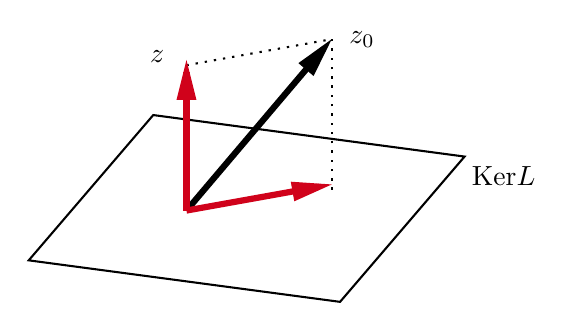
\begin{tikzpicture}[x=0.75pt,y=0.75pt,yscale=-1,xscale=1]
                      %uncomment if require: \path (0,152); %set diagram left start at 0, and has height of 152

                      %Straight Lines [id:da7968494763005547] 
                      \draw [color={rgb, 255:red, 0; green, 0; blue, 0 } ,draw opacity=1 ][line width=0.75]  [dash pattern={on 0.84pt off 2.51pt}]  (256,26) -- (326,13.44) ;
                      %Shape: Polygon [id:ds47696393353033595] 
                      \draw   (330,140) -- (180,120) -- (240,50) -- (390,70) -- cycle ;
                      %Straight Lines [id:da04367598648625459] 
                      \draw [line width=2.25]    (256,96) -- (322.12,18.01) ;
                      \draw [shift={(326,13.44)}, rotate = 490.29] [fill={rgb, 255:red, 0; green, 0; blue, 0 }  ][line width=0.08]  [draw opacity=0] (19.2,-4.8) -- (0,0) -- (19.2,4.8) -- cycle    ;
                      %Straight Lines [id:da8880773272488094] 
                      \draw [color={rgb, 255:red, 208; green, 2; blue, 27 } ,draw opacity=1 ][line width=2.25]    (256,96) -- (320.09,84.5) ;
                      \draw [shift={(326,83.44)}, rotate = 529.8299999999999] [fill={rgb, 255:red, 208; green, 2; blue, 27 } ,fill opacity=1 ][line width=0.08]  [draw opacity=0] (19.2,-4.8) -- (0,0) -- (19.2,4.8) -- cycle    ;
                      %Straight Lines [id:da3687846316598724] 
                      \draw [color={rgb, 255:red, 208; green, 2; blue, 27 } ,draw opacity=1 ][line width=2.25]    (256,96) -- (256,29.44) ;
                      \draw [shift={(256,23.44)}, rotate = 450] [fill={rgb, 255:red, 208; green, 2; blue, 27 } ,fill opacity=1 ][line width=0.08]  [draw opacity=0] (19.2,-4.8) -- (0,0) -- (19.2,4.8) -- cycle    ;
                      %Straight Lines [id:da07890995266380374] 
                      \draw [color={rgb, 255:red, 0; green, 0; blue, 0 } ,draw opacity=1 ][line width=0.75]  [dash pattern={on 0.84pt off 2.51pt}]  (326,86) -- (326,13.44) ;

                      % Text Node
                      \draw (392,73.4) node [anchor=north west][inner sep=0.75pt]    {$\mathrm{Ker} L$};
                      % Text Node
                      \draw (333,8.4) node [anchor=north west][inner sep=0.75pt]    {$z_{0}$};
                      % Text Node
                      \draw (237,17.4) node [anchor=north west][inner sep=0.75pt]    {$z$};


                  \end{tikzpicture}

              \end{figure}
              \FloatBarrier


              Scegliamo quindi $H,V=\mathrm{Ker} L,x=z_{0}$, dobiamo verificare che $V$ è un sottospazio chiuso topologicamente per applicare le proiezioni.
              \begin{itemize}
                  \item È un sottospazio, vogliamo dimostrare che
                        \begin{equation*}
                            v_{1},v_{2} \in \mathrm{Ker} L\ \ \Rightarrow \ \ \lambda _{1} v_{1} +\lambda _{2} v_{2} \in \mathrm{Ker} L
                        \end{equation*}

                        ovvero che
                        \begin{equation*}
                            Lv_{1} =Lv_{2} =0\ \ \Rightarrow \ \ L(\lambda _{1} v_{1} +\lambda _{2} v_{2}) =0
                        \end{equation*}

                        ma per \textbf{linearità} di $L$ è soddisfatta
                        \begin{equation*}
                            L(\lambda _{1} v_{1} +\lambda _{2} v_{2}) =\lambda _{1} Lv_{1} +\lambda _{2} Lv_{2} =0
                        \end{equation*}
                  \item Che sia chiuso è leggermente più delicato, osserviamo intanto che per definizione
                        \begin{equation*}
                            \text{chiuso} \ \ \Leftrightarrow \ \ \left\{
                            \begin{array}{ l }
                                (v_{n})_{n} \subset \mathrm{Ker} L \\
                                v_{n}\rightarrow \overline{v} \in H
                            \end{array} \Rightarrow \overline{v} \in \mathrm{Ker} L\right\}
                        \end{equation*}nel nostro caso
                        \begin{equation*}
                            (v_{n})_{n} \subset \mathrm{Ker} L\ \ \Leftrightarrow \ \ Lv_{n} =0
                        \end{equation*}è vero che $L\overline{v} =0$? Sì grazie alla \textbf{continuità}.
              \end{itemize}

              Allora possiamo applicare il teorema delle proiezioni
              \begin{equation*}
                  z=\frac{z_{0} -P_{\mathrm{Ker} L} z_{0}}{\Vert z_{0} -P_{\mathrm{Ker} L} z_{0}\Vert }
              \end{equation*}con questa scelta, si ha $\boxed{z\in (\mathrm{Ker} L)^{\perp }}$ e $\Vert z\Vert =1$. Abbiamo
              \begin{equation*}
                  v\in H\ \ \ \ z\in (\mathrm{Ker} L)^{\perp }
              \end{equation*}costruiamo $\boxed{w\in \mathrm{Ker} L}$ che sia combinazione di quei due
              \begin{equation*}
                  w=v-\frac{Lv}{Lz} z\ \ \Rightarrow \ \ Lw=L\left(v-\frac{Lv}{Lz} z\right) =Lv-\frac{Lv}{Lz} Lz=0
              \end{equation*}Notiamo che dato che $w\in \mathrm{Ker} L,z\in (\mathrm{Ker} L)^{\perp }$ allora $(w,z) =0$, pertanto
              \begin{equation*}
                  0=(w,z) =\left(v-\frac{Lv}{Lz} z,z\right) =(v,z) -\frac{Lv}{Lz}\underbrace{(z,z)}_{\Vert z\Vert ^{2} =1}
              \end{equation*}infine
              \begin{equation*}
                  Lv=Lz(z,v) =(\underbrace{(Lz) z}_{u},v),\ \ \forall v\in H
              \end{equation*}
    \end{itemize}

    \textit{Unicità.}

    Supponiamo che questo vettore $u$ non sia unico, cioè che ne esistano due $u_{1},u_{2} \in H$ tali che
    \begin{gather*}
        (u_{1},v) =Lv,\ \forall v\in H\\
        (u_{2},v) =Lv,\ \forall v\in H
    \end{gather*}
    sottraiamo membro a membro
    \begin{equation*}
        (u_{1} -u_{2},v) =0,\ \ \forall v\in H
    \end{equation*}
    questo implica che $u_{1} -u_{2} =0$.\footnote{Questa ultima implicazione non può essere fatta con troppa leggerezza, infatti siamo in uno spazio astratto e l'unica cosa che abbiamo sono le definizioni e i teoremi. Il fatto che quella cosa valga per ogni $v$, significa in particolare che vale anche per $v=u_{1} -u_{2}$, degli altri infiniti $v$ non ci interessa. Con tale scelta
    \begin{equation*}
        0=(u_{1} -u_{2},u_{1} -u_{2}) =\Vert u_{1} -u_{2}\Vert ^{2}
    \end{equation*}
    Per la proprietà di annullamento della norma
    \begin{equation*}
        \Vert u_{1} -u_{2}\Vert ^{2} =0\ \ \Leftrightarrow \ \ u_{1} -u_{2} =0
    \end{equation*}
    Alternativamente per la proprietà di annullamento del prodotto scalare
    \begin{equation*}
        (u_{1} -u_{2},u_{1} -u_{2}) =0\ \ \Leftrightarrow \ \ u_{1} -u_{2} =0
    \end{equation*}}
\end{dimostrazione}
\begin{definition}
    La scrittura $a:H\times H\rightarrow \mathbb{R}$ denota una \textbf{forma bilineare} se
    \begin{itemize}
        \item fissato $u$,
              \begin{equation*}
                  v\mapsto a(u,v) \ \ \text{è lineare in} \ v
              \end{equation*}
        \item fissato $v$,
              \begin{equation*}
                  u\mapsto a(u,v) \ \ \text{è lineare in} \ u
              \end{equation*}
    \end{itemize}
\end{definition}
\begin{definition}
    Inoltre
    \begin{itemize}
        \item $a$ si dice \textbf{simmetrica} se

              \begin{equation*}
                  a(u,v) =a(v,u),\ \ \forall v,u\in H
              \end{equation*}

              in generale non lo sarà, ma un esempio ne è il prodotto scalare.
        \item $a$ si dice \textbf{continua} (\textbf{limitata}) se

              \begin{equation*}
                  \exists M:\ \ | a(u,v)| \leqslant M\Vert u\Vert \Vert v\Vert,\ \ \forall v,u
              \end{equation*}
        \item $a$ si dice \textbf{coerciva/coercitiva} se

              \begin{equation*}
                  \exists \alpha  >0\ \text{(costante di coercività)} :\ \ a(u,u) \geqslant \alpha \Vert u\Vert ^{2}
              \end{equation*}
    \end{itemize}
\end{definition}
Segnaliamo una domanda che ogni tanto viene fatta agli orali di Salsa: nella continuità e nella coercività serve il modulo nella forma bilineare?

Se siamo nei numeri complessi, sempre in entrambe, altrimenti la quantità non sarebbe correttamente definita per una disuguaglianza.
Se siamo nei numeri reali, come da definizione non serve per la coercività, ma in realtà non serve nemmeno nella continuità, infatti certamente quella col modulo implica quella senza modulo, ma quella senza modulo implica quella col modulo:
\begin{align*}
    a(u,v)\le M \Vert u \Vert \Vert v \Vert,\ \forall u,v \quad \Rightarrow \quad a(-u,v) & \le  M \underbrace{\Vert -u \Vert}_{\Vert u \Vert} \Vert v \Vert \\
    -a(u,v)                                                                               & \le  M \Vert u \Vert \Vert v \Vert                               \\
    a(u,v)                                                                                & \ge -M \Vert u \Vert \Vert v \Vert,
\end{align*}
che messe assieme implicano quella col modulo.\footnote{Uno degli autori del documento si è giocato la lode (non la laurea) su questa domanda, quindi studiatela.}

Il prodotto scalare è un caso particolare di forma bilineare simmetrica $a(u,v) =(u,v)$, vediamo quanto valgono le costanti $M$ e $\alpha $. Per Cauchy-Schwarz
\begin{equation*}
    | (u,v)| \leqslant \Vert u\Vert \Vert v\Vert \ \ \Rightarrow \ \ M=1
\end{equation*}
Per definizione di norma indotta dal prodotto scalare
\begin{equation*}
    (u,u) =\Vert u\Vert ^{2} \ \ \Rightarrow \ \ \alpha =1
\end{equation*}
Il teorema di Lax-Milgram generalizza queste nozioni e ci permette di risolvere\footnote{esistenza, unicità e dipendenza continua.} il seguente problema.
\begin{definition}
    [Problema Variazionale Astratto, \eqref{eq:pva}] Dato $L\in H^{*}$ trovare $u\in H$ tale che
    \begin{equation}
        \tag{PVA}
        a(u,v) =Lv,\ \ \forall v\in H
        \label{eq:pva}
    \end{equation}
    dove $a$ è una forma bilineare.
\end{definition}
Nel caso di prodotto scalare $a(u,v) =(u,v)$, \eqref{eq:pva} diventa $(u,v) =Lv$ che è ben posto per il teorema di Riesz.
\subsection{Teorema di Lax-Milgram}
\begin{theorem}
    [di Lax-Milgram] Siano
    \begin{itemize}
        \item $H$ spazio di Hilbert
        \item $a$ forma bilineare \textbf{continua} e \textbf{coerciva}
        \item $L\in H^{*}$
    \end{itemize}

    Allora $\exists !\ \overline{u} \in H$ soluzione di \eqref{eq:pva}. Inoltre (\textbf{stima di stabilità})
    \begin{equation*}
        \Vert \overline{u}\Vert \leqslant \frac{1}{\alpha }\Vert L\Vert _{*}
    \end{equation*}
    dove $\alpha $ è la costante di coercività, ci interessa che sia più grande possibile.
\end{theorem}
\begin{oss}
    La stabilità è utile considerando due dati vicini e due soluzioni vicine. Prendiamo ad esempio due soluzioni $u_{1},u_{2}$ soluzioni del \eqref{eq:pva} coi dati $L_{1} v,L_{2} v$
    \begin{gather*}
        a(u_{1},v) =L_{1} v,\ \ \forall v\in H\\
        a(u_{2},v) =L_{2} v,\ \ \forall v\in H
    \end{gather*}
    Facciamo la differenza e usiamo la linearità
    \begin{equation*}
        a(u_{1} -u_{2},v) =(L_{1} -L_{2}) v
    \end{equation*}
    La stima di stabilità ci dice che
    \begin{equation*}
        \Vert u_{1} -u_{2}\Vert \leqslant \frac{1}{\alpha }\Vert L_{1} -L_{2}\Vert _{*}
    \end{equation*}
    Ovvero a \textit{dati vicini} sono associate \textit{soluzioni vicine}, a patto che $\alpha $ sia sufficientemente grande.
\end{oss}
\begin{dimostrazione}
    Proponiamo un'overview dei passi della dimostrazione
    \begin{enumerate}
        \item[(0)] Riscrittura del problema in termini di $A$
        \item[(1)] $A$ è lineare
        \item[(2)] $A$ è continuo (ovvero limitato)
        \item[(3)] $A$ è iniettivo (ovvero $\mathrm{Ker} A=\{0\}$)
        \item[(3.5)] l'immagine $R(A)$ è un sottospazio chiuso, cosa \textbf{non} vera in generale
        \item[(4)] $A$ è suriettivo (ovvero $R(A) =H$)
    \end{enumerate}
    Procediamo quindi con la dimostrazione
    \begin{itemize}
        \item[(0)]

              Notiamo che la $v$ è una sorta di \textit{funzione test}, infatti vogliamo ottenere una cosa che vale per infiniti $v$. Al secondo membro del \eqref{eq:pva}, per ipotesi $L\in H^{*}$, allora per Riesz $\exists !\ z\in H$ tale che $Lv=(z,v),\forall v$ e inoltre $\Vert z\Vert =\Vert L\Vert _{*}$. Vogliamo applicarlo anche al primo membro. Per definizione di forma bilineare, $\forall u$ fissato, l'applicazione $v\mapsto a(u,v)$ è lineare e inoltre per ipotesi continua in $v$:
              \begin{equation*}
                  \text{continua} \ \ \Leftrightarrow \ \ | a(u,v)| \leqslant \underbrace{M\Vert u\Vert }_{C}\Vert v\Vert \leqslant C\Vert v\Vert
              \end{equation*}
              allora per Riesz per ogni $u$ fissato $\exists !\ h=A(u) \in H$ tale che
              \begin{equation*}
                  a(u,v) =(h,v),\ \ \forall v
              \end{equation*}
              cioè ho definito un'applicazione $A:H\rightarrow H$ tale che
              \begin{equation*}
                  \boxed{a(u,v) =(A(u),v),\ \forall v\in H}
              \end{equation*}
              noi vogliamo dimostrare su $A$, ma abbiamo proprietà su $a$, questa relazione è la \textbf{chiave!}

              Avendo così usato due volte il teorema di Riesz per passare da due operatori lineari a due prodotti scalari, il \eqref{eq:pva} diventa
              \begin{equation*}
                  (A(u),v) =(z,v) \ \ \forall v\in H
              \end{equation*}
              Sottraiamo membro a membro e deduciamo, con la proprietà di annullamento del prodotto scalare
              \begin{equation*}
                  (A(u) -z,v) =0,\ \forall v\in H\ \ \Rightarrow \ \ \boxed{A(u) =z}
              \end{equation*}
              risolvere \eqref{eq:pva} quindi \textit{è come} trovare l'operatore \textit{inverso} di $A$.

        \item[(1)]

              Dobbiamo sempre lavorare con il prodotto scalare di $A$ per qualcosa, in modo da usare la chiave trovata al passo precedente
              \begin{equation*}
                  (A(\lambda u_{1} +\mu u_{2}),v) =a(\lambda u_{1} +\mu u_{2},v) =(*)
              \end{equation*}
              da qui è tutto automatico
              \begin{align*}
                  (*) & =\lambda a(u_{1},v) +\mu a(u_{2},v)                    \\
                      & =\lambda (A(u_{1}),v) +\mu (A(u_{2}),v)                \\
                      & =(\lambda A(u_{1}) +\mu A(u_{2}),v) \ \ \forall v\in H
              \end{align*}
              cioè $A(\lambda u_{1} +\mu u_{2}) =\lambda A(u_{1}) +\mu A(u_{2})$.

              D'ora in poi useremo la \textbf{notazione}
              \begin{equation*}
                  A(u) =Au
              \end{equation*}

        \item[(2)]

              Notiamo che
              \begin{equation*}
                  \Vert Au\Vert ^{2} =(Au,Au) =a(u,Au) \leqslant | a(u,Au)| \leqslant M\Vert u\Vert \Vert Au\Vert
              \end{equation*}
              l'ultima maggiorazione grazie al fatto che $a$ è limitata; allora
              \begin{equation*}
                  \Vert Au\Vert \leqslant M\Vert u\Vert
              \end{equation*}
              Se $\Vert Au\Vert $ fosse stato $0$ non avrei avuto nulla dimostrare, per cui ho potuto semplificare.

        \item[(3)]

              È l'unico in cui non possiamo mettere il pilota automatico. Qui troveremo anche la \textbf{stima di stabilità}. Per farlo dobbiamo partire dalla coercività
              \begin{equation*}
                  \alpha \Vert u\Vert ^{2} \leqslant a(u,u) =(Au,u) \leqslant | (Au,u)| \underbrace{\leqslant }_{\text{C.S.}}\Vert Au\Vert \Vert u\Vert \ \ \alpha  >0
              \end{equation*}
              Possiamo dividere per $u$ perché se fosse $0$ sarebbe soddisfatta già, otteniamo la stima di stabilità
              \begin{equation*}
                  \Vert u\Vert \leqslant \frac{1}{\alpha }\Vert Au\Vert
              \end{equation*}
              Nel nuovo \eqref{eq:pva} $Au=z$ e ricordiamo che $z$ era il vettore che rappresentava $L$ (come visto al passo 0)
              \begin{equation*}
                  \Vert u\Vert \leqslant \frac{1}{\alpha }\Vert Au\Vert =\frac{1}{\alpha }\Vert z\Vert =\frac{1}{\alpha }\Vert L\Vert _{*}
              \end{equation*}
              Se $u\in \mathrm{Ker} A$ allora $Au=0$, usando la stima $\Vert u\Vert \leqslant 0$, allora $u=0$. Quindi $\mathrm{Ker} A=\{0\}$, ovvero $A$ è iniettivo.

        \item[(3.5)]

              L'immagine è un sottospazio, analogo a come visto prima.

              Dimostriamo che è chiuso, ovvero che considerando ogni successione contenuta nell'immagine $(y_{n})_{n} \subset R(A)$ che tende a un certo valore $y_{n}\rightarrow \overline{y}$ allora quel valore sta nell'immagine $\overline{y} \in R(A)$\footnote{ricordiamo che la definizione è \textit{interessante} se consideriamo i punti del bordo in particolare.}.

              Questi valori dell'immagine sono associati agli elementi del dominio $y_{n} =Au_{n}$, ci piacerebbe dire che $\overline{y} =A\overline{u}$, con $\overline{u} =\lim u_{n}$, \textbf{ma questo limite non è detto che esista! In un sacco di situazioni concrete salta!}

              Ci rivolgiamo nuovamente alla completezza dello spazio, dimostrando che è una successione di Cauchy, usando la stima di stabilità del passo (3)
              \begin{equation*}
                  0\leqslant \Vert u_{n} -u_{m}\Vert \underbrace{\leqslant }_{(3)}\frac{1}{\alpha }\Vert A(u_{n} -u_{m})\Vert \underbrace{\leqslant }_{\text{lin.}}\frac{1}{\alpha }\Vert Au_{n} -Au_{m}\Vert =\frac{1}{\alpha }\Vert y_{n} -y_{m}\Vert
              \end{equation*}
              la successione $y_{n}$ è convergente, quindi anche di Cauchy, allora l'ultimo termine tende a $0$, in particolare quindi anche $u_{n}$ è di Cauchy, ma essendo $H$ completo è anche convergente a un certo $\overline{u} \in H$.

              Usando la continuità di $A$, $Au_{n}\rightarrow A\overline{u}$, quindi $\overline{y} =A\overline{u} \in R(A)$.

        \item[(4)]

              Supponiamo per assurdo che
              \begin{equation*}
                  R(A) \varsubsetneqq H
              \end{equation*}
              cioè esiste $z_{0} \in H$, $z_{0} \notin R(A)$. Per il teorema delle proiezioni\footnote{che possiamo applicare avendo dimostrato che l'immagine $R(A)$ è un sottospazio chiuso al passo (3.5)}
              \begin{equation*}
                  z=\frac{z_{0} -P_{R(A)} z_{0}}{\Vert z_{0} -P_{R(A)} z_{0}\Vert } \ \ \Rightarrow \ \ z\in (R(A))^{\perp },\ \Vert z\Vert =1
              \end{equation*}
              A questo punto notiamo che
              \begin{equation*}
                  z\in (R(A))^{\perp },\ \ Az\in R(A) \ \ \Rightarrow \ \ (z,Az) =0
              \end{equation*}
              Andando alla definizione di $A$ e usando la coercività
              \begin{equation*}
                  (z,Az) =a(z,z) \geqslant \alpha \Vert z\Vert ^{2} =\alpha  >0
              \end{equation*}
              Ma ciò è assurdo, è quindi negata la supposizione iniziale e $R(A) =H$.
    \end{itemize}
\end{dimostrazione}